\documentclass[a4paper,12pt]{article}
\usepackage[total={6in, 8in}, margin=1.2in, bottom=1in]{geometry}
\usepackage{amsmath}
\usepackage{bera}
\usepackage{indentfirst}
%\usepackage{enumitem}
\usepackage{multirow}
\usepackage{graphicx}
\usepackage{csquotes}
%\usepackage{float}
\usepackage[font=normalsize]{caption}
\usepackage{subcaption}
\usepackage{floatrow}
%\setlength{\parindent}{-1em}
\usepackage[formats]{listings}
\usepackage{color}
\renewcommand\lstlistingname{Quelltext} % Change language of section name
\lstset{ % General setup for the package
	language=C++,
	basicstyle=\small\sffamily,
	%numbers=left,
 	%numberstyle=\tiny,
 	tabsize=5,
	frame=t,
	framesep = 3pt,
	framextopmargin = 6pt,
	columns=fixed,
	showstringspaces=false,
	showtabs=false,
	keepspaces,
	commentstyle=\color{green},
	keywordstyle=\color{blue}
}
\begin{document}

\renewcommand\thesection{\arabic{section}}
\renewcommand\thesubsection{\thesection.\arabic{subsection}}

\section {\textbf{Mathematical formulae and notations (15 marks)}}
%
\subsection{\textbf{Equation Array (4 marks)}}
%
\begin{eqnarray}
cos^3\theta + sin^3\theta & = & (cos\theta + sin\theta)(cos2\theta - cos\theta sin\theta)\\
& = & (cos\theta + sin\theta)(1 - cos\theta sin\theta)\\
& = & (cos\theta + sin\theta)(1/2)(2 - 2cos\theta sin\theta)(3)\\
& = & (1/2)(cos\theta + sin\theta)(2 - sin(2\theta))
\end{eqnarray}
%\textbf{(1)}

\subsection {\textbf{Prepositional Formulae using Various Operators (2 marks)}}
%
\begin{flalign*}
(\exists x)(\varphi(x) \wedge \psi(x)) & \longleftrightarrow ((\exists x)\varphi(x)\wedge (\exists x)\psi(x)) & \\
\medskip
(\exists x)(\varphi(x) \wedge \psi(x)) & \longrightarrow ((\exists x)\varphi(x) \wedge (\exists x)\varphi(x) \wedge (\exists x)\psi(x))
\end{flalign*}

\subsection {\textbf{Alphabets (3 marks + 1 mark for table)}}
%
\begin{center}
\begin{tabular}{|c|c|}
\hline
Binary Operators: & $\times$ $\otimes$ $\oplus$ $\cup$ $\cap$ \\
&\\
\hline
Relation Operators: & $\subset$ $\supset$ $\subseteq$ $\supseteq$ < > \\
&\\
\hline
Others: & $\int$ $\oint$ $\sum$ $\prod$\\
&\\
\hline
\end{tabular}
\end{center}

\subsection {\textbf{Mathematical Formulas (5 marks)}}
%
\begin{enumerate}%
\item $ \int_a ^b x^3 dx = \frac{1}{4}x^4\Big\rvert_a ^b $
\item $ \frac{\pi}{4} =  4\sum\limits_{n=0}^{\infty} \frac{(-1)^n}{(2n+1)5^{2n+1}}  -  \sum\limits_{n=0}^{\infty} \frac{(-1)^n}{(2n+1)239^{2n+1}} $
\item $ \pi = \frac{3\sqrt{3}}{4} -24\sum\limits_{n=0}^{\infty} \frac{\frac{(2n)!}{n}}{2n+1(2n+1)239^{2n+1}} $
\item $\frac{1}{\pi} = \frac{2\sqrt{2}}{9801}\sum\limits_{n=0}^{\infty}\frac{(4n)!(1103 + 26390n)}{(n)!^4396^{4n}} $
\item $\sum_{i=0}^{[\frac{n}{2}]} \binom{x^{i^2}_{i,i+1}}{[\frac{i+3}{3}]} = \frac{\sqrt{\mu(i)^{\frac{3}{2}}(i^2 - 1)}}{\sqrt[3]{\rho(i)-2}+\sqrt[3]{\rho(i)-1}}$
\end{enumerate}
\pagebreak

\section{\textbf{Tables (10 marks)}}
%
\noindent To combine rows a package must be imported with in your preamble, then you can use the XXXXXXX command in your document. The table below includes mathematical notations, which you can produce by embedding the expression in \$ \$ delimiters. For subscript, use underscore and for superscript, use carrot.
\newline
\begin{table}[H]
\centering
\resizebox{\columnwidth}{!}{
\begin{tabular}{|c|c|c|c|c|c|c|c|c|c|c|}
\cline{3-11}
\multicolumn{2}{c}{} & \multicolumn{5}{|c}{\textbf{Basic Properties}} & \multicolumn{4}{|c|}{\textbf{Readability}} \\
\cline{3-11}
\multicolumn{2}{c|}{} & \textbf{WC} & \textbf{SC} & \textbf{C-W} & \textbf{S-W} & \textbf{W-S} & \textbf{FK} & \textbf{GF} & \textbf{SMOG} & \textbf{LEX} \\
\hline
\multirow{2}{6em}{\textit{Baseline}} & Mean & 0.84 & 0.41 & \textbf{0.56} & \textbf{0.46} & \textbf{0.55} & \textbf{0.60} & 0.56 & 0.57 & 0.63 \\
\cline{2-11}
& SD & 0.07 & 0.08 & 0.06 & 0.07 & 0.05 & 0.05 & 0.06 & 0.07 & 0.05 \\
\hline
\hline
\multirow{2}{6em}{\textit{ScaComp\textsubscript{h}}} & Mean & 0.89 & 0.46 & 0.53 & 0.43 & 0.53 & 0.58 & 0.54 & 0.56 & 0.62 \\
\cline{2-11}
& SD & 0.05 & 0.08 & 0.05 & 0.06 & 0.06 & 0.05 & 0.05 & 0.06 & 0.05 \\
\hline
\hline
\multirow{2}{6em}{\textit{ScaComp\textsubscript{t}}} & Mean & \textbf{0.92} & {\bf 0.48} & 0.55 & 0.45 & 0.53 & 0.59 & {\bf 0.58} & {\bf 0.61} & {\bf 0.64} \\
\cline{2-11}
& SD & 0.04 & 0.07 & 0.05 & 0.04 & 0.05 & 0.04 & 0.04 & 0.04 & 0.04 \\
\hline

%    a & b & c & d  \\
 %   e & f & g & h 
\end{tabular}   
}
\captionsetup{width = 0.9\textwidth, font=normalsize}
\caption{Table depicting the use of both multirow and multicolumn}
\end{table}
{\Large In table 1 above, we try to demonstrate all the features required to be demonstrated in a table.  We use multiple newline, we use a package to enable the use of multiple rows,  and multiple columns in the table.Additionally,  We have also drawn lines from specific column to column.   We also use box resizing with a width specifier for resizing the box within the limits of the document, and avoid any overflow.}
\pagebreak
\section{\textbf{Image Insert (7 + 7 marks)}}
\setlength{\parindent}{1cm} Now, we will import images side by side in the same document.\\

\begin{figure}[H]
    \centering
    \begin{floatrow}
      \ffigbox[\FBwidth]{\caption{Screenshot: Mobile Interface}\label{fig:dummy-1}}{%
       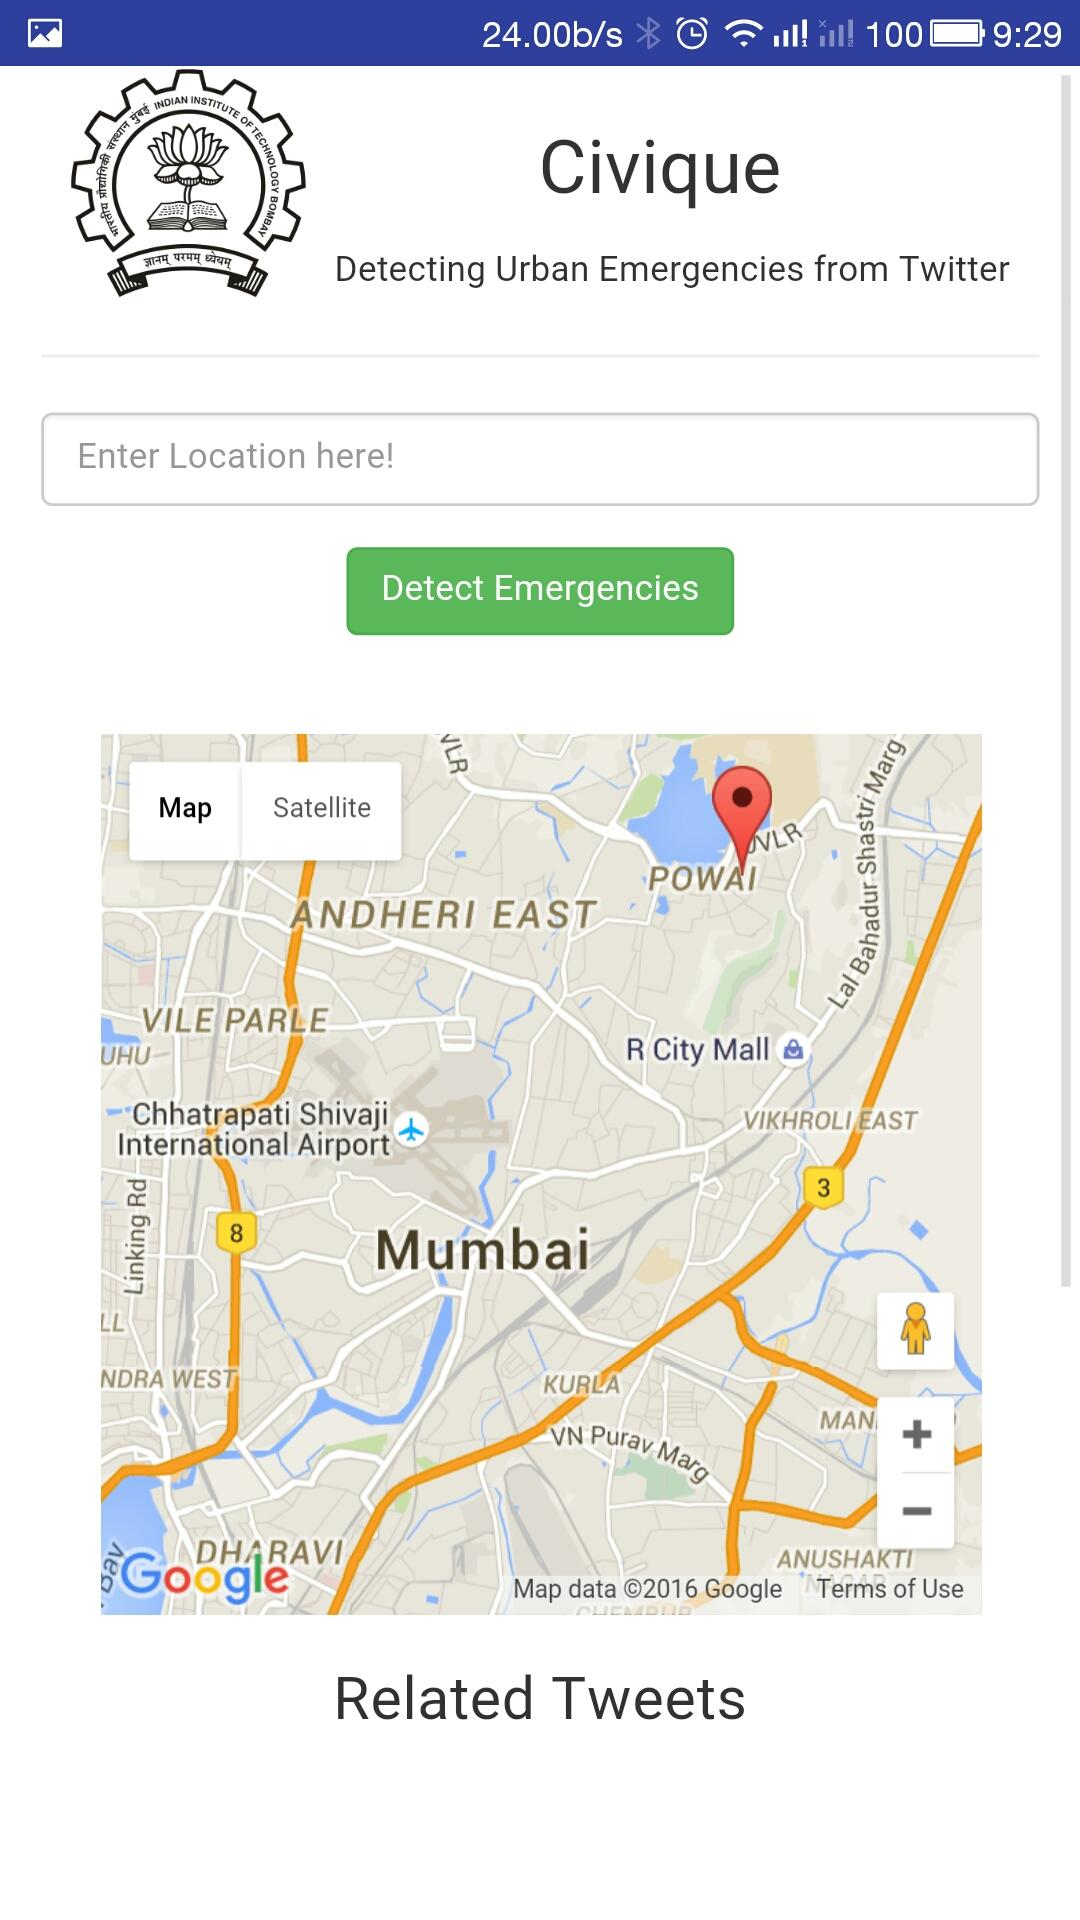
\includegraphics[width=6cm]{1.jpg}   % Just a dummy. Replace with your figure.
      }
      \ffigbox[\FBwidth]{\caption{ Screenshot: Generated Notification}\label{fig:dummy-2}}{%
        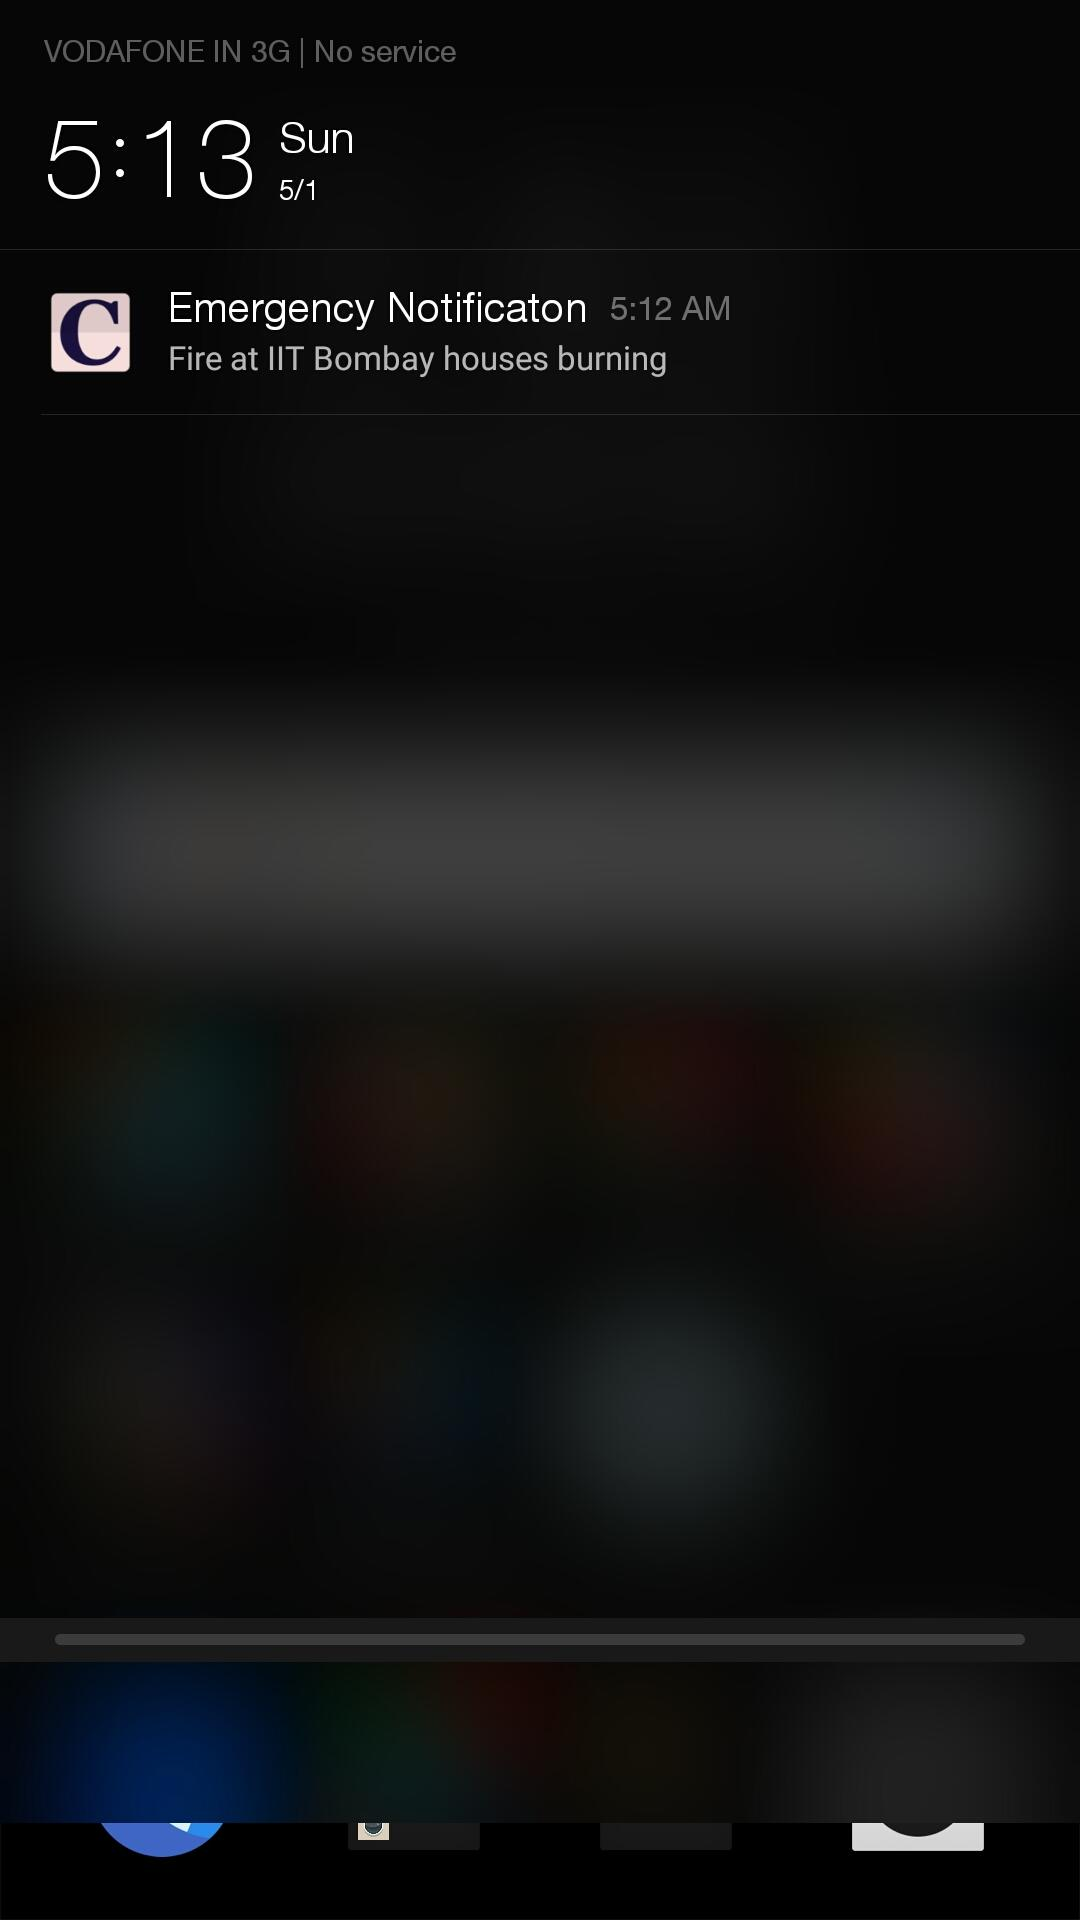
\includegraphics[width=6cm]{2.jpg}   % Just a dummy. Replace with your figure.
      }
    \end{floatrow}
  \end{figure}
 \setlength{\parindent}{1em}
The images have been put in, and they are side by side in the same document on the same page. We have used the package {\bf floatrow} and {\bf graphicx} to import images on Page 6.
\par In case you would like to see an alternative method to align the images, for instance images as subfigures, here it is.
\begin{figure}[H]
\centering
\begin{subfigure}{.5\textwidth}
  \centering
  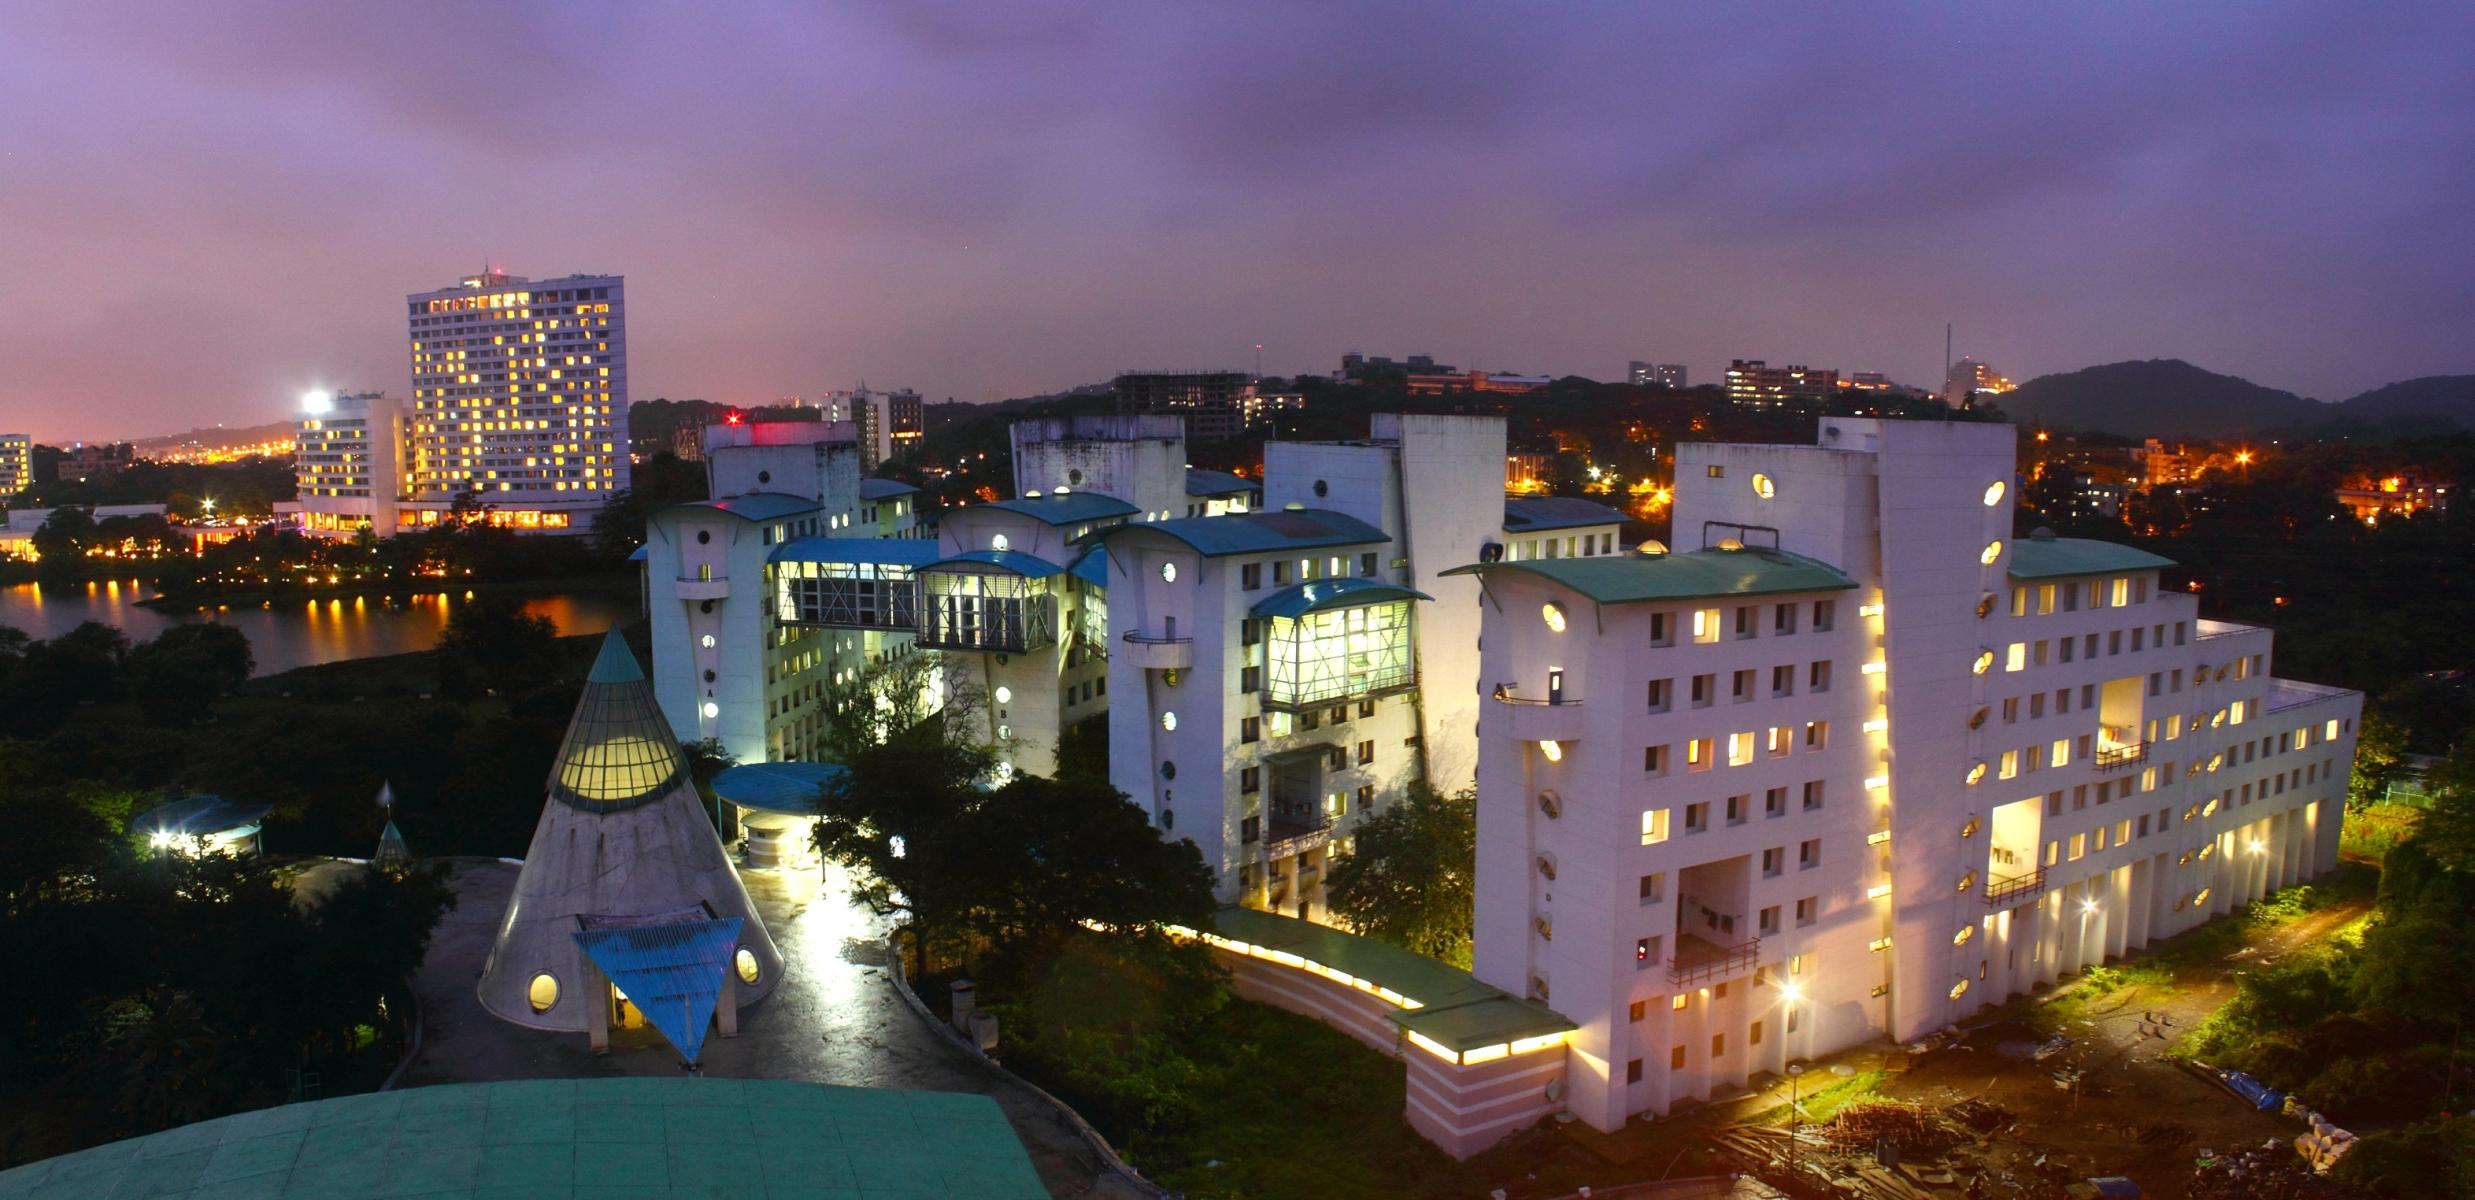
\includegraphics[width=.9\linewidth, height = 4.4cm]{3.jpg}
  \caption{Caption1}
  \label{fig:sub1}
\end{subfigure}%
\begin{subfigure}{.5\textwidth}
  \centering
  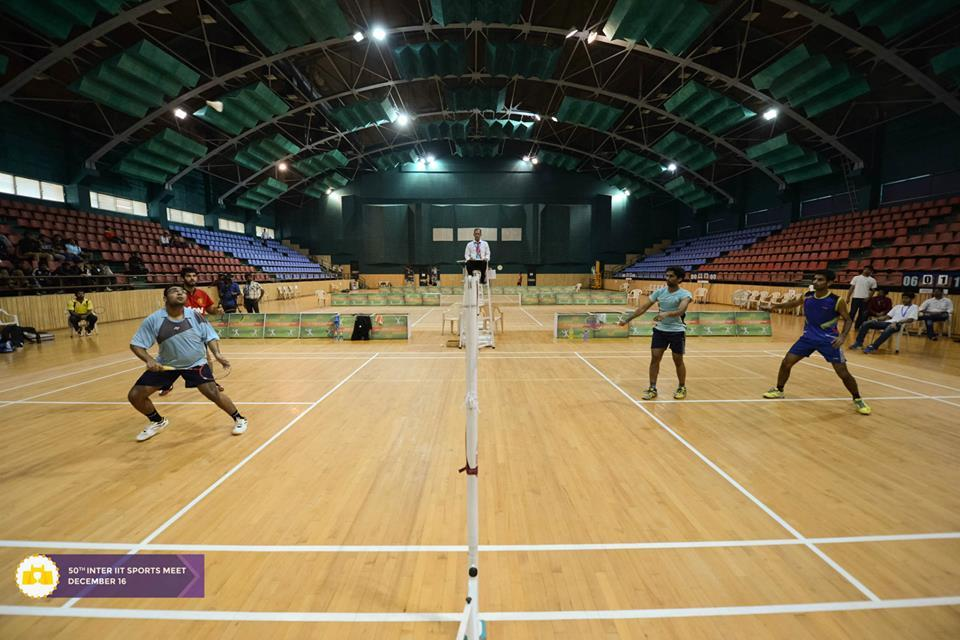
\includegraphics[width=.9\linewidth]{4.jpg}
  \caption{Caption2}
  \label{fig:sub2}
\end{subfigure}
\caption{Caption for this figure with two images}
\label{fig:test}
\end{figure}
\pagebreak
\section{\textbf{Quotaion and Citation (4 marks)}}
\subsection{Quotation (2 marks)}
\noindent The margins of the quotation environment are indented on both the left and the right. The text is justified at both margins. Leaving a blank line between text produces a new paragraph. The package \textbf{csquotes} offers a multilingual solution to quotations, with integration to citation mechanisms offered by BibTeX.This package allows one for example to switch languages and quotation styles according to babel language selections.\\
\setquotestyle[american]{english}
\begin{displayquote}
\enquote{Unlike the quote environment, each paragraph is indented normally. It's important to remark that even if you are typing quotes on English there are different quotation marks used in English (UK) and English(US).}
\end{displayquote}
\subsection{Citation (2 marks)}
Latex \cite{ref1} is a document preparation system for typesetting program. It is used to create different types of document structures. A Latex file (.tex) is created using any text editor (vim, emacs, gedit, etc.).  There are also many LaTeX IDEs like Kile, TexStudio, etc.. The Latex code is then compiled which creates a standard (.pdf) file. Thus, the presentation of the document does not change on different machines.\\
Type style\cite{ref2} is used to indicate logical structure. Emphasized text appears in italic style type and input in typewriter style. Type style is specified by three components: shape, series, and family.\\
\par There are two ways of producing a bibliography\cite{ref3}. You can either produce a bibliography by manually listing the entries of the bibliography or producing it automatically using the BibTeX program of LaTeX. The bibliography style can be declared with bibliography style command, which may be issued anywhere after the preamble. The style is a file with .bst extension that determines how bibliography entries will appear at the output, such as if they are sorted or not,or how they are labeled etc. The extension .bib is not written explicitly. There are many standard bibliography style files. Two of them that are compatible with IIT thesis manual are plain.bst and alpha.bst. They are part of the LaTeX package; a student does not need to download it. The plain.bst and alpha.bst styles are explained below. The symbols in a math formula fall into different classes that correspond more or less to the part of speech each symbol would have if the formula were ex pressed in words. Certain spacing and positioning cues are traditionally used for the different symbol classes to increase the readability of formulas. \cite{ref4}
\par My citations are in proper order as per references ref1, ref2, ref3, and ref4.

\pagebreak
\section{\textbf{Algorithm and Pseudo Code (22 marks)}}
\subsection{\textbf{Listing (10 marks)}}
\begin{lstlisting}
//Breadth First Search Function
void BFS(list<long long int>queue,long long int length
    ){
     long long int v;
     if(queue.empty())
         return; 
     list<long long int>::iterator i;
     list<long long int>queue_temp;
     while(!queue.empty()){
          v=queue.front();
          queue.pop_front();
          for(i=adj[v].begin();
               i!=adj[v].end();i++){
               if(!pro_ver[*i]){
                    result[*i]=length;
                    queue_temp.push_back(*i);
                    pro_ver[*i]=true;
                    adj[*i].remove(v);
               }
          }
     }
     BFS(queue_temp,length+1);
}
\end{lstlisting}
\pagebreak
\begin{thebibliography}{9}
\bibitem{ref1} a
\bibitem{ref2} b
\bibitem{ref3} c
\bibitem{ref4} d

\end{thebibliography}
\end{document}
